\section{Experimental Setup}
\label{sec:setup}

\subsection{Datasets}
Three public corpora are used (Table~\ref{tab:data}); Fig.~\ref{fig:workflow} outlines the study. In each, the two
modalities come from the same individual and are paired at the source rather
than by a construction rule, which a claim about fusion requires. They also
cover the two regimes that matter for the mechanism: clients holding many
individuals (VitalDB, eICU) and a client holding one (WEAR). WEAR is not
clinical: it is a wearable IoT workload that tests the system objectives
outside medicine, and its privacy results are record-level.

\begin{figure*}[!t]
\centering
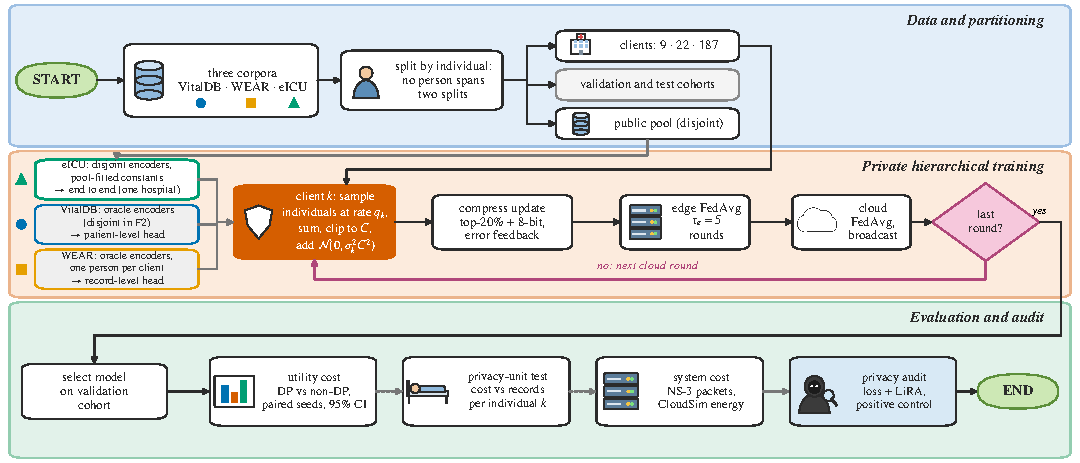
\includegraphics[width=\textwidth]{fig00_workflow.pdf}
\caption{Study workflow: individual-level partitioning, per-corpus encoder configuration (end to end on eICU only), private hierarchical training and paired evaluation with an attack audit.}
\label{fig:workflow}
\end{figure*}

\emph{VitalDB} \cite{ref20} contains non-cardiac surgical cases. Modality~A
is ten minutes of nine intraoperative trends at $0.5$~Hz with nine binary
indicators of whether each was recorded; modality~B is a $34$-dimensional
vector of preoperative clinical and laboratory variables. The target is
postoperative intensive-care admission. Clients are the nine surgical
specialties, which differ by a factor of almost eight in size and by more than
fifteen in outcome prevalence ($3.0$--$50.4\,\%$ on the person-level
partition; $3.2$--$50.7\,\%$ on the case-level partition), a
heterogeneity that arises from how care is organized rather than from an
imposed skew. \emph{WEAR} \cite{ref21}
combines body-worn inertial sensing with egocentric video features
synchronized in hardware; each of the $22$ clients is one participant.
\emph{eICU} \cite{ref27}, distributed through PhysioNet \cite{ref28} under a
credentialed agreement, is the external clinical corpus. Modality~A is the
first $24$ hours after unit admission in $60$-minute windows of six vital signs
and six observation indicators; modality~B is age, sex, admission weight and
height and the APACHE score, a clinician-computed summary rather than an
independent sensor stream; the target is in-unit mortality. Prediction is
made at hour $24$: individuals who die within the first $24$ hours are
excluded, and the APACHE score, computed from the worst values of the first
day, is therefore available at prediction time. Clients are the
hospitals themselves: of $206$, those with fewer than $200$ windows or no
positive outcome are pooled, giving $187$ clients with a median of $444$
individuals.

\begin{table}[!t]
\centering
\caption{The three corpora}
\label{tab:data}
\setlength{\tabcolsep}{2.6pt}
\small
\begin{tabular}{lccc}
\toprule
& VitalDB & WEAR & eICU \\
\midrule
Clients     & $9$ specialties & $22$ participants & $187$ hospitals \\
Ind.        & $5{,}974$ & $22$ & $132{,}736$ \\
Windows (k) & $33.5/6.8/6.9$ & $26.4/5.4/6.0$ & $2122/564/570$ \\
$\bar{k}$   & $7.9$ & ${\approx}1{,}750$ & $28.5$ \\
Modality A  & $18$-ch.\ trends & $12$-ch.\ inertial & $12$-ch.\ vitals \\
Modality B  & $34$ preop. & $2048$ video & $5$ admission \\
Task        & ICU admission & $18$ activities & mortality \\
Prevalence  & $18.84\,\%$ & -- & $4.22\,\%$ \\
\bottomrule
\end{tabular}
\tabnote{Ind.: individuals; $\bar{k}$: mean records per individual; windows are
training/validation/test, in thousands. VitalDB: person-level partition (the
case-level partition has $6{,}257$ cases, $34.0/7.3/7.4$k windows and a
prevalence of $19.65\,\%$).}
\end{table}

On eICU and WEAR, splits are made by individual. VitalDB is evaluated on two
partitions. The \emph{person-level} partition assigns each person to one
split and one client; cases that would place a person in a second split or on
a second client are removed ($200$ cases), leaving $4{,}221$ training, $868$
validation and $885$ test persons. The \emph{case-level} partition of the
earlier experiments splits by operation, so that $55$ of $940$ test persons
also have a training case and $68$ training persons span two clients; results
on it protect the case rather than the person and are marked case-level. The
privacy cost, the cost of the unit, the comparison with prior systems and the
membership-inference audit are person-level. All partitions are fixed, and no test case of either was used to
pretrain the encoders. Four controls prevent inflation that would
not be visible during training: splits by case rather than by window, which
would place near-duplicates in the test set; modality~B restricted to
preoperative variables, because intraoperative interventions are given in
response to deterioration and encode the outcome; missing values filled
within a case and paired with an explicit indicator, because, for example, an
arterial line is placed only in patients judged at risk; and normalization
statistics computed on training cases only, or on the disjoint pool for the
end-to-end eICU run. For eICU, a pool of $526{,}867$
windows from individuals disjoint from every client is reserved before
federated training to pretrain the disjoint encoders.

\subsection{Implementation}
Table~\ref{tab:params} lists the training and evaluation parameters. All arms
share one configuration, so that differences can be attributed to the factor
under test. The headline system uses per-client multipliers and the privacy
loss distribution accountant (Section~\ref{sec:method:calib}). On eICU every
pretrained encoder is disjoint. On VitalDB and WEAR, results use the oracle
encoders unless stated, so absolute utilities there are upper bounds, whereas
differences between arms, which share the encoders, are unaffected. The
trained model is exported to ONNX and timed with ONNX Runtime on the CPU
provider of a workstation (Intel Core i7-14700), not on edge hardware; the network is simulated in ns-3 and energy is modeled in
CloudSim~Plus.

\begin{table}[!t]
\centering
\caption{Training and evaluation parameters}
\label{tab:params}
\footnotesize
\setlength{\tabcolsep}{4pt}
\begin{tabular}{@{}p{0.40\columnwidth}p{0.56\columnwidth}@{}}
\toprule
Parameter & Value \\
\midrule
Cloud rounds $R$; edge rounds $\tau_e$ & $10$; $5$ \\
Edge aggregators $E$ & $2$ (eICU scaling test: $2$--$16$) \\
Local passes per edge round & $1$ \\
Optimizer & Adam \\
Learning rate; weight decay & $10^{-3}$; $10^{-4}$ \\
Expected individuals per step $B$ & $64$ \\
Clipping norm $C$ & $1$ \\
Training budget & $\varepsilon = 0.9$, $\delta = 10^{-5}$ \\
Accountant & privacy loss distribution, per-client $\sigma_k$ \\
Records per patient (cap) & $64$ \\
Update encoding & top-$20\,\%$, $8$-bit, error feedback \\
Seeds & $5$ (paired); $3$ for grids \\
LiRA shadow models & $16$ \\
Latency timing & P95, $1{,}000$ runs, $100$ warm-up \\
Software & PyTorch~2.5, Opacus~1.5, ONNX Runtime, ns-3~3.46, CloudSim~Plus~8.5 \\
Hardware & one NVIDIA RTX~A2000 GPU \\
\bottomrule
\end{tabular}
\end{table}

\subsection{Metrics and Statistics}
The primary utility measure is the area under the ROC curve (AUROC); average
precision (AUPRC) is reported because the clinical tasks are imbalanced.
Accuracy at the default threshold is uninformative under this imbalance: a
constant negative prediction attains the base rate. Balanced accuracy is
therefore reported at a threshold chosen on the validation cohort by Youden's
index. Case-level metrics average the predictions of a case's windows.
Comparisons between arms are paired by seed, and intervals are
\begin{equation}
\bar d \pm t_{S-1,\,0.975}\; s_d / \sqrt{S}
\label{eq:ci}
\end{equation}
over $S$ seeds with per-seed differences $d_s$. An effect is called
\emph{resolved} when this interval excludes zero; an unresolved estimate is
reported as such and is not read as evidence of absence. Grids run at three
seeds estimate how a cost changes across a factor, not each cell
individually. Seed counts were fixed before
each comparison and were not increased after inspecting results. The
reported checkpoint is the one with the best validation AUROC, and each is
evaluated once on the test split.

\subsection{Experimental Protocol}
\emph{System objectives} compare PP-HFM with centralized training and with the
hierarchy alone. \emph{Privacy cost} (O2b) compares the private system with
an identical non-private system over five paired seeds; the primary measure
(AUROC) and the secondary measures (AUPRC, balanced accuracy) were declared
before the runs. \emph{Recipe decomposition} uses three arms at
$\varepsilon \in \{0.5, 1, 2, 4, 8, \infty\}$: B4, full-model private training
from random initialization (prior art); B7, full-model private training from
the pretrained initialization; and B6, head-only private training from the
pretrained initialization (PP-HFM). B4$\rightarrow$B7 changes only the
initialization and B7$\rightarrow$B6 only the privatized subset.
\emph{Records per individual}: the number of training records retained per
individual, $k$, is varied with the number of units per step held equal in
both arms, which removes the sampling-rate effect and leaves only the
clipping geometry; validation and test sets are unchanged, and $k = 1$ is the
control of Corollary~\ref{cor:k1}. \emph{Ablations} remove one component at a
time. \emph{Fusion} is measured outside the federated system, each arm
retrained on its own inputs, because zeroing a stream of a jointly trained
model measures robustness rather than information.
